\documentclass[tikz]{standalone}
\usepackage{tikz}
\usepackage[compat=1.0.0]{tikz-feynman}
\begin{document}
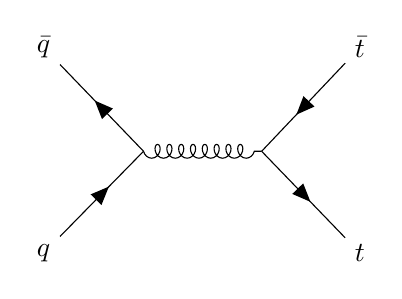
\begin{tikzpicture}
  \begin{feynman}
    \vertex (a);
    \vertex [right = of a] (b);
    \vertex [below right=of b] (f2) {\(t\)};
    \vertex [above right=of b] (f1) {\(\bar{t}\)};
    \vertex [below left=of a] (i2) {\(q\)};
    \vertex [above left=of a] (i1) {\(\bar{q}\)};
    \diagram* {
        (i2) -- [fermion] (a) -- [fermion] (i1),
        (a) -- [gluon] (b),
        (f1) -- [fermion] (b) -- [fermion] (f2),
        };
  \end{feynman}
\end{tikzpicture}

\end{document}